\chapter{Introduction}

\section{Motivation}

Emotion analysis is one of the fastest growing research areas of the last
couple
decades. More than 99\% of the papers regarding sentiment analysis are from
after 2004 \cite{MANTYLA201816}. There have been multiple articles published
comparing different approaches for emotion detection. The most recent and
comprehensive one I found being \cite{REUSENS2024124302}. However this article
not only focuses in emotion detection but on text classification in general.
Since it is a review and the models compared were not run with equivalent
hardware, time comparison for training and inference is impossible. It also
does not compare rule based systems.

This research is motivated by the lack of direct comparison in both performance
(F1 score, precision, accuracy, recall) and computation time of rule based
emotion detection, vanilla neural networks (NN) and more complex NN
architectures (LSTM, RoBERTa, etc). The goal is to provide new insights into
the costs of training and running these models so that better decisions can be
made when trying to deploy them for commercial applications. That is why this
study asks, \textit{Are the performance improvements of more complex and
    computationally expensive models worth the cost?}

\section{Emotion detection approaches}

This study will focus on three specific approaches to emotion detection. These
being rule based systems, vanilla neural networks and more complex neural
network architectures, specifically Long Short Term Memory (LSTM) networks.

\subsection{Rule based systems}

Rule based systems are the oldest approach to emotion detection. They are based
on a set of rules that are used to determine the emotion of a given text. These
rules are usually based on the presence of specific words or phrases that are
associated with a specific emotion. The most famous model representing these
relationships is the OCC model \cite{ortony2022cognitive} where the different
dimensions such as tense, direction, polarity, etc. are used to determine the
emotion of a given text. Rule based systems are usually very fast and can be
easily implemented. However, they are limited by the fact that they rely on a
predefined set of rules and are not able to learn from new data. This means
that they are not able to adapt to new types of text or new emotions that may
not be covered by the rules.

\subsection{Neural Networks}

Vanilla neural networks are a type of machine learning model that is inspired
by the human brain. They consist of nodes (neurons) that are
connected to each other in a network. Each node takes an input, processes it,
and passes the output to the next node in the network. The output of the final
node in the network is the prediction made by the model.

Neural networks are considered to be universal function approximators
\cite{hornik1989multilayer}. They are able to learn any function given enough
data and computational power. Neural networks are able to
learn from new data and adapt to new types of text or new emotions. However,
they are usually slower than rule based systems and require more computational
power to train.

Vanilla neural networks have some disadvantages when processing text.They have
fixed length inputs and outputs, meaning the same model would either be unable
to process long sequences or waste resources processing smaller ones. There are ways
around this problem like pooling results but this looses the order of the
words in the text.

\subsection{Beyond vanilla neural networks}

Recurrent Neural Networks (RNN) are a type of neural network that is able to
process sequences of data. They are able to remember information from previous
time steps in the sequence and use it to make predictions about future time
steps (fig \ref{fig:unfolded_rnn}). This makes a good fit for tasks like
emotion detection where the order and correlation of the words in the text is
important. However, they still have limitations as back propagation through
time can lead to vanishing or exploding gradients. Effectively making long term
dependencies impossible to learn \cite{hochreiter1997long}.

\begin{figure}[!ht]
    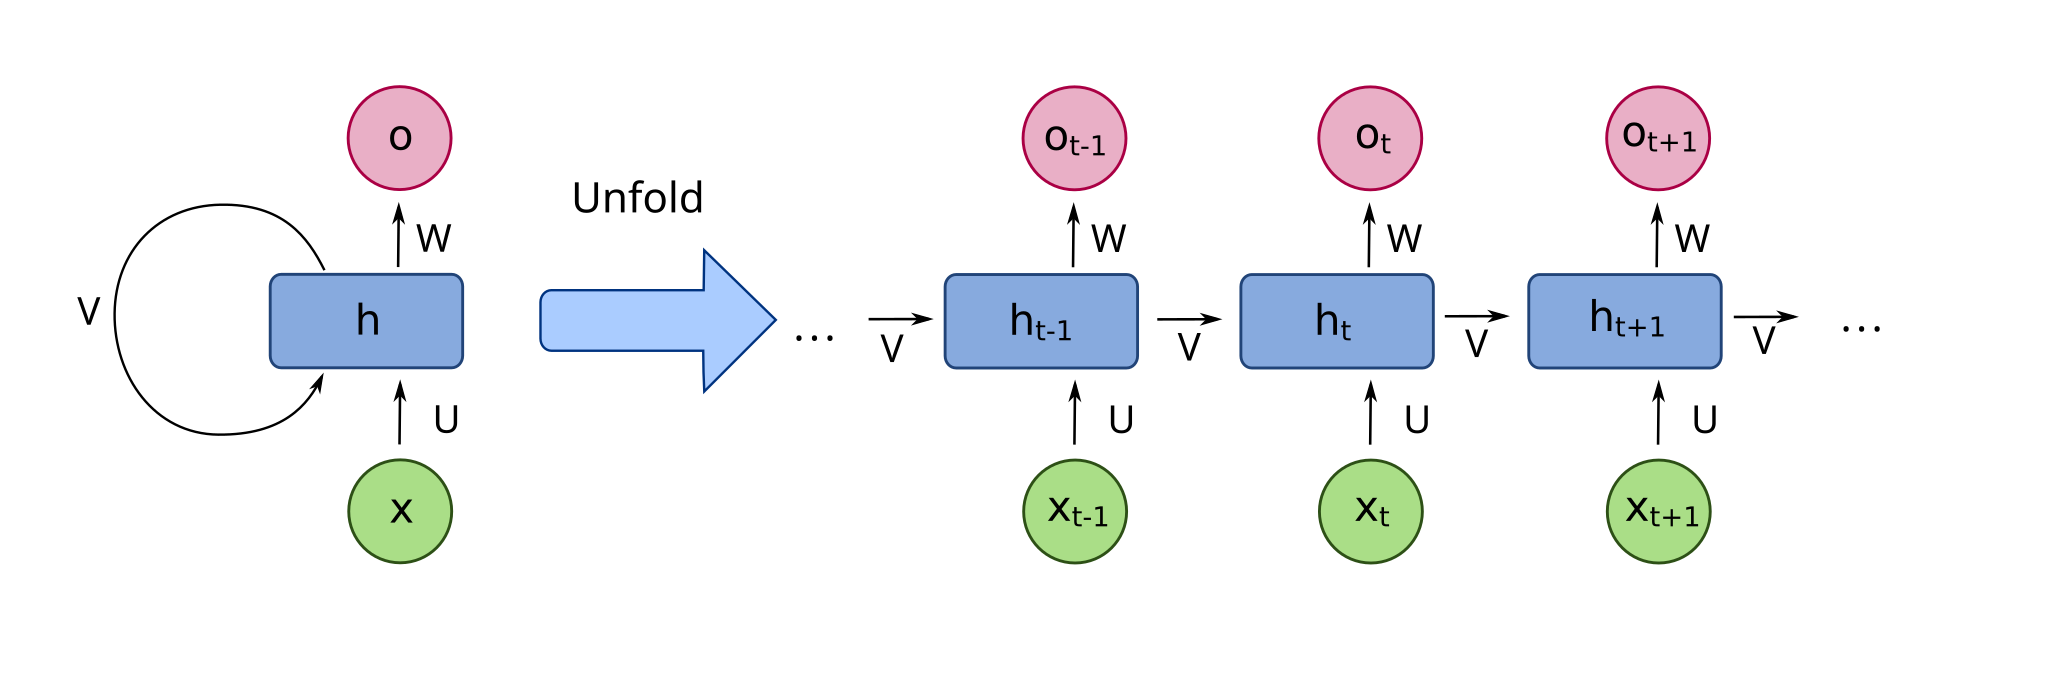
\includegraphics[keepaspectratio,
        width=15cm]{./figures/2048px-Recurrent_neural_network_unfold.png}
    \caption{Unfolded RNN \cite{RNN}}
    \label{fig:unfolded_rnn}

\end{figure}

Here is where Long Short-Term Memory (LSTM) networks come in. They are a type
of
RNN that is able to learn long term dependencies in the data. They are able to
remember information from previous time steps and use it to make predictions
about future time steps. This is done by using a series of gates (fig
\ref{fig:lstm_unit}) that guarantee that the gradients do not vanish or
explode. This makes them well suited for tasks such as emotion detection, where
the order of the words in the text is important.

\begin{figure}[!ht]
    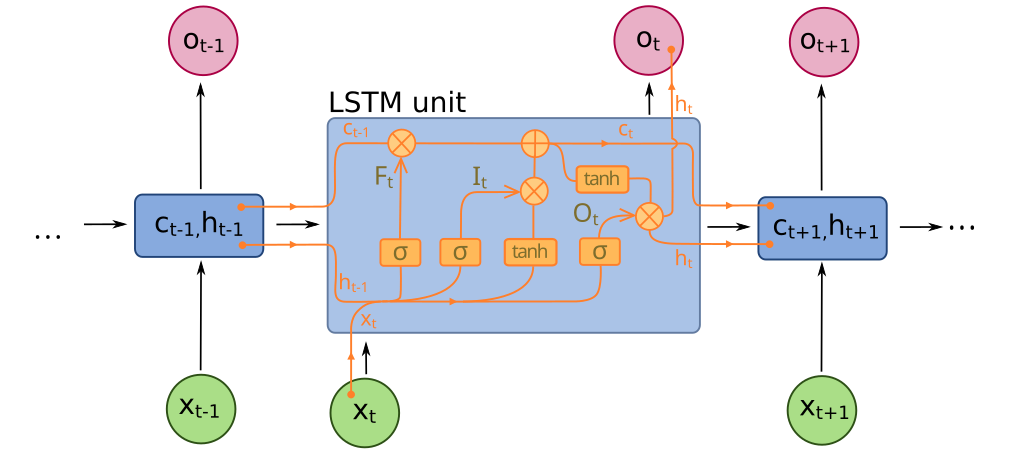
\includegraphics[keepaspectratio,
        width=15cm]{./figures/1024px-Long_Short-Term_Memory.png}
    \caption{LSMT unit \cite{LSTM}}
    \label{fig:lstm_unit}

\end{figure}